\section{Design}
\subsection{Decisions} 
When the prestydy was completed it was time to make some decisions about the content of the platform, how it should look and how different parts should be implemented. To give a picture of how the design on the user interface should look like, a group sketched some simple mockups
so that every member could have the same starting point and vision. 

\begin{figure}[H]
  \centering
  \begin{minipage}[b]{0.7\textwidth}
    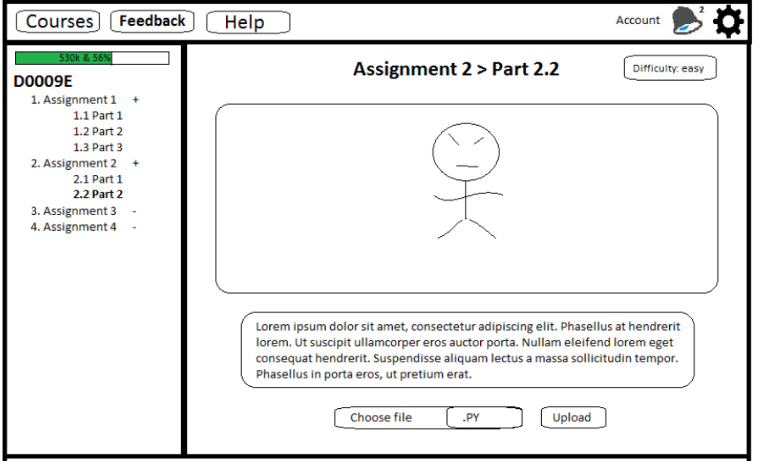
\includegraphics[width=\textwidth]{img/mockup1.png}
    \caption{An initial mockup over the assignment page.}
  \end{minipage}
  \hfill
  \begin{minipage}[b]{0.7\textwidth}
    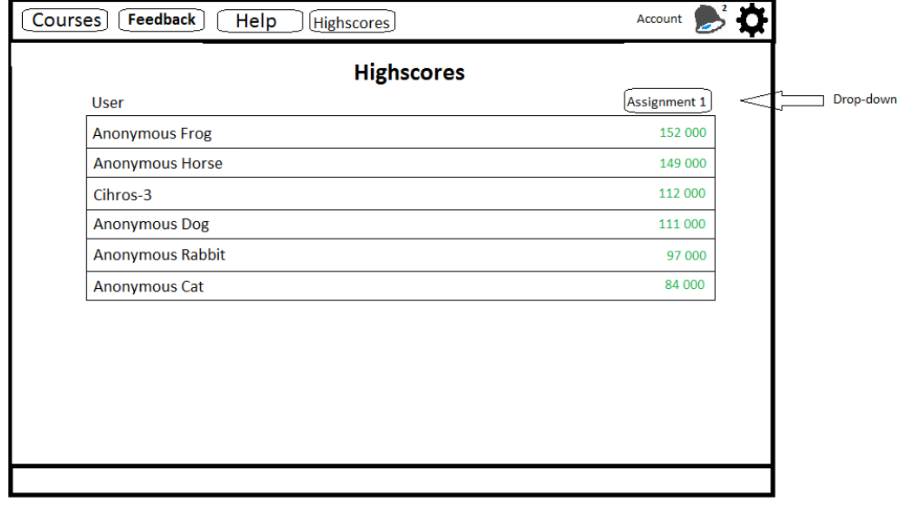
\includegraphics[width=\textwidth]{img/mockup2.png}
    \caption{An initial mockup over the leaderboard.}
  \end{minipage}
\end{figure}

The mockups were only used to have a base and the rest of the design would grown during the implementation time and it was mostly the frontend group that designed the pages. 
During the prestudy it become clear that the whole system flow was needed to be implemented. No one of the found an existing solution that would fit with the system and it couldn't be ensured that it will work over time. The system was divided into three parts. Tester whose main task was to implement a system that is able to test code that students write and send back some feedback. The frontend should implement the user interface and the gamification visualization. The backend is the in the middle and it will take the code from frontend and load a test from the database, send the submitted code along with the tests to Tester and then give the response (feedback) back to the frontend.

\begin{figure}[H]
\centering
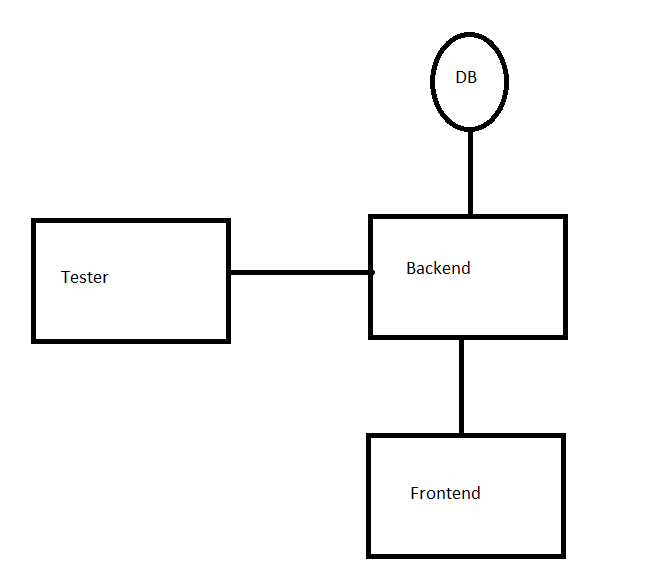
\includegraphics[scale=0.8]{img/SystemA.png}
\caption{A simple sketch over the system parts and how they are connected.}
\end{figure}

The time estimation for every separate part was difficult to estimate since the concept was fairly new for everyone. The decision of what programming language to use was based on the criteria, it should be fullstack meaning the same language should be used in every part so that if there is any interaction between the three groups it should be easy to understand the code. It should also be fairly modern programming language. The two alternatives was Python with frameworks or JavaScript with other frameworks. A democratic choice become JavaScript using Node.Js for backend and Tester, MongoDB as a NoSQL database and Angular4 for frontend. 


\subsection{Use-cases}
In the system there are two different roles, teacher and student. The teacher is able to create courses, assignments and invite students to the courses. The student can solve assignments.
Students who want to solve an assignment go to the site, log in, go to the specific assignment and write the code required in the assignment and submit it. The code is sent to the backend that saves the code to the database for future changes and loads the tests that belong to the assignment from the database. It then sends both the tests and the code to Tester which tests the code and sends back the output through the backend which in turn calculates the correct number of points that the student should be given for their solution. The output is now served to the frontend and the student can see if the code has passed or not with feedback.


\subsection{Frontend}
\begin{figure}[H]
\centering
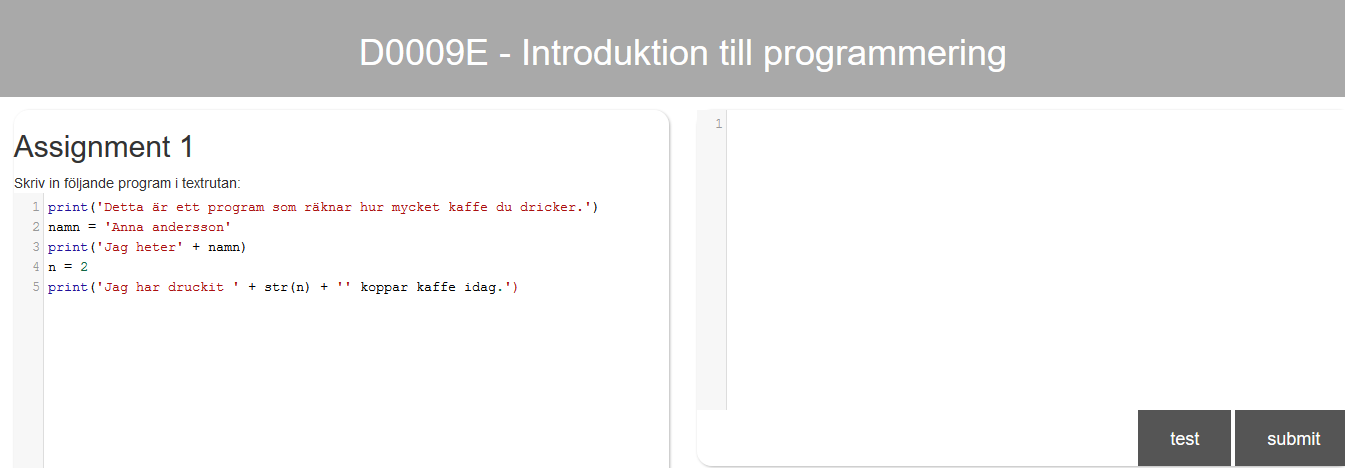
\includegraphics[scale=0.45]{img/Codemirror_pic.png}
\caption{A screenshot over how assignment looked when using codemirror.}
\end{figure}
\begin{figure}[H]
\centering
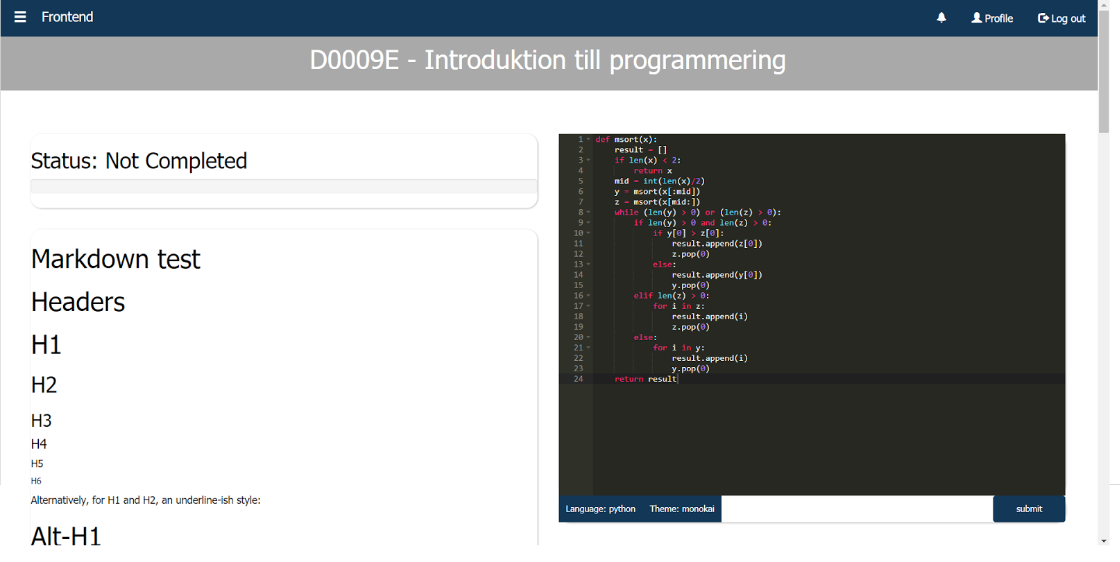
\includegraphics[scale=0.5]{img/Ace.png}
\caption{A screenshot over how assignment looked when using Ace. }
\end{figure}
\begin{figure}[H]
\centering
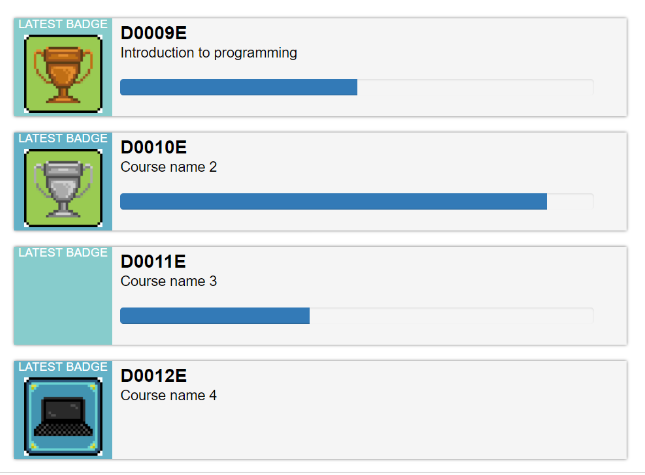
\includegraphics[scale=0.6]{img/Progress.png}
\caption{How the progress and badges look like.}
\end{figure}

\subsection{Backend}
A backend group was formed after all the prestudies were finished.
Beginning to work on the backend, the first decision that had to be made was what it was going to be developed in. Since it had been decided previously that the project would be a full-stack JavaScript solution the natural decision was to use node.js as server framework with express.js as a web framework to handle routing, for database it was decided to use the document database MongoDB.

The first few days were mostly spent on getting acquainted with node.js and its work flow.
After the group had gotten a general grasp of things, a coding standard was decided on and the group was divided into sub-parts in the backend.
The parts that the group was divided into were routes, database and continuous integration.
\\
It was decided that it was very important for continuous integration to be a part of the project. The reasoning for using continuous integration was that having a modern workflow where you could push changes to git and have them available on a live test server would be important to keep the project effective. Using continuous integration was also a good way to effectively separate production and development builds and a way to ensure that production builds always kept a certain standard and robustness.
However, while the idea and reasoning for using continuous integration was good, the concept wasn't put to as good use as it could have been. For the first half of the project, the continuous integration wasn't really used they way it was intended too, mainly due to communication errors and the fact that it wasn't needed as much, but for the second part of the project it was used more.

\subsection{Tester}
